\usepackage{cite}
\usepackage{polski}
\usepackage[utf8]{inputenc}
\usepackage{array}
\usepackage{hyperref}
\usepackage{graphicx}
\usepackage{listings}

\date{10 IV 2018}

\usetheme{AGH}
\title{Binutils, Biblioteki statyczne i dynamiczne }
\author{Robert Gałat}

\institute[AGH] % (optional)
{
  Wydział Fizyki i Informatyki Stosowanej\\
  Akademia Górniczo-Hutnicza im. Stanisława Staszica
}
 \usepackage{adjustbox}

\title{Binutils, biblioteki dynamiczne i statyczne} \author{Gabriel Górski}
\date{10 IV 2018} \institute[AGH]{
  Wydział Fizyki i Informatyki Stosowanej\\
}

%%%%%%%%%%%%%%%%% 
\begin{document}


\maketitle
\part{Pliki obiektowe}
%%%%%%%%%%%%%%%% 
\begin{frame}{Zarys}
  \tableofcontents
\end{frame}
%%%%%%%%%%%%%%%% 
\section{Wstęp}
\begin{frame}{Wstęp}
  Kod maszynowy który procesor \textit{umie ewaluować} jest fundamentalną acz
  nie jedyną częścią pliku obiektowego.\\

  Plik obiektowy --- aby był użyteczny --- musi zawierać w sobie wszelkie
  informacje konieczne do tego by dało się go integrować z innymi plikami
  obiektowymi i ostatecznie doprowadzić do formy wykonywalnej.
\end{frame}
%%%%%%%%%%%%%%%% 
\section{Sposób reprezentacji}
%%%%%%%%%%%%%%%% 
\begin{frame}{Formaty plików}
  Konieczna jest jakaś fizyczna, udokumentowana manifestacja pliku obiektowego
	tj. \textbf{format}\\

  Przykłady formatów plików obiektowych
  \begin{block}{ELF}
    Executable and Linkable Format (więcej przy okazji analizy)
  \end{block}
  \begin{exampleblock}{PE}
    Portable Executable
  \end{exampleblock}
  \begin{alertblock}{Mach-O}
    Mach object
  \end{alertblock}
\end{frame}
%%%%%%%%%%%%%%%% 
\begin{frame}{Rodzaje plików obiektowych}
  Rodzaje plików obiektowych w ramach formatu ELF:
  \begin{enumerate}
  \item Relocatable object
  \item Executable object
  \item Shared object
  \item Core object
  \end{enumerate}
\end{frame}
\begin{frame}{Relocatable object}
  Jest to bezpośredni efekt pracy kompilatora który musi zostać poddany dalszemu
  linkowaniu. Zawiera \textit{luki} które muszą zostać poddane procesowi
  relokacji w czasie linkowania (stąd nazwa).\\
	Może powstać w wyniku łączenia przez linker kilku innych plików tego typu.\\
	\textbf{Przykład}
  \begin{exampleblock}{}
    plik.c $\rightarrow$ kompilator $\rightarrow$ plik.o
  \end{exampleblock}
\end{frame}
\begin{frame}{Executable object}
  Efekt procesu linkowania. Zawiera wszystkie konieczne informacje do wykonania
  programu. Wszystkie adresy są już odpowiednio zmapowane lub jest zawarta
  informacja o konieczności dostarczenia odpowiednich symboli poprzez spełnienie
  zależności wobec odpowiednich współdzielonych bibliotek \textbf{Przykład}
  \begin{exampleblock}{}
    {plik1.o, plik2.o, plik3.o ...} + [-lbiblioteka1 -lbiblioteka2 ...]
    $\rightarrow$ linker $\rightarrow$ plik.out
  \end{exampleblock}
\end{frame}

\begin{frame}{Shared object, core object}
  \begin{itemize}
  \item \textbf{Shared object}\\
    Efekt linkowania przy opcji \textit{--shared}. Typ pliku wykorzystywany jako
    biblioteka współdzielona lub współcześnie bardzo często jak plik
    wykonywalny. Więcej przy porównaniu typów bibliotek
  \item \textbf{Core object}\\
    Plik obiektowy będący zrzutem obrazu procesu w momencie jego śmierci w
    wyniku błędu.
  \end{itemize}
\end{frame}
%%%%%%%%%%%%%%%% 
\part{Biblioteki}
\begin{frame}{Zarys}
  \tableofcontents
\end{frame}
\section{Wstęp}
\begin{frame}{Typy bibliotek}
  Wyróżniamy dwa typy bibliotek
  \begin{itemize}
  \item Biblioteki statyczne
  \item Biblioteki współdzielone
  \end{itemize}
\end{frame}
\section{Biblioteki statyczne}
\begin{frame}[allowframebreaks]{Biblioteki statyczne}
  Biblioteka statyczna jest archiwum plików obiektowych które możemy zlinkować z
  naszymi plikami źródłowymi. Tak powstały plik wykonywalny będzie już potem w
  pełni niezależny. \textbf{Przykład}\\

  Działanie:
  \begin{itemize}
  \item Proces linkowania zaczyna się od podanych plików obiektowych. Powstaje w
    ten sposób lista brakujących symboli będących zależnościami
  \item Kolejno podane biblioteki statyczne są rozpatrywane od lewej do prawej
	\item Linkowane są jedynie te pliki obiektowe (z bibliotek)
    które dostarczają brakujących symboli ze wspomnianej listy
  \item Ma to swoje konsekwencje: jeśli w liście podanych linkerowi argumentów
    biblioteka B znajduje się za biblioteką A, a biblioteka B korzysta z symboli
    z \textbf{niedołączonego} pliku obiektowego z biblioteki A to nastąpi błąd
    linkowania
  \end{itemize}
  Wnioski:
  \begin{itemize}
  \item Kolejność bibliotek w liście argumentów ma znaczenie
  \item Może wystąpić cykliczna zależność
  \end{itemize}
\end{frame}
%%%%%%%%%%%%%%%% 
\begin{frame}{Tabela pomocnicza do przykładu}
  \adjustbox{max height=\dimexpr\textheight-5.5cm\relax, max width=\textwidth}{
    \begin{tabular}{|l|l|l|l|l|l|}
      \hline
      &                          & \multicolumn{3}{c}{Biblioteka A}                                          & Biblioteka B        \\
      \hline
      Pliki obiektowe                                & staticlibraryusage.o     & add2num.o         & dostuff.o                         & uselessfunction.o & anotherfunction.o   \\
      \hline
      Dostarczane referencje                          & main                     & add2num, what     & dostuff                           & uselessfunction   & anotherfunction     \\
      \hline
      Brakujące referencje                           & anotherfunction, add2num & anotherfunction   &                                   &                   & dostuff             \\
      \hline
      Lista brakujących referencji L $\rightarrow$ P & anotherfunction, add2num & anotherfunction   & anotherfunction                   & anotherfunction   & dostuff             \\
      \hline
      &                          & Biblioteka B      & \multicolumn{3}{c}{Biblioteka A}                                            \\
      \hline
      Pliki obiektowe                                & staticlibraryusage.o     & anotherfunction.o & add2num.o                         & dostuff.o         & uselessfunction.o   \\
      \hline
      Dostarczane referencje                          & main                     & anotherfunction   & add2num, what & dostuff           & uselessfunction     \\
      \hline
      Brakujące referencje                           & anotherfunction, add2num & dostuff           & anotherfunction                   &                   &                     \\
      \hline
      Lista brakujących referencji L $\rightarrow$ P & anotherfunction, add2num & add2num, dostuff  & dostuff                           &                   &   \\ 
      \hline
    \end{tabular}
  }
\end{frame}
%%%%%%%%%%%%%%%% 
\section{Biblioteki współdzielone}
\begin{frame}{Biblioteki współdzielone}
  W odróżnieniu od bibliotek statycznych będących jedynie archiwami plików
  obiektowych, \textbf{biblioteki współdzielone} wprowadzają zupełnie nowy mechanizm.\\
  
  Linkowanie względem obiektu współdzielonego (shared object) powoduje zawarcie
  w wynikowym pliku wykonywalnym \textbf{informacji o odpowiedniej
    zależności/zależnościach}, która ma
  być rozwiązana \textbf{w momencie uruchomienia programu}.\\

  Zadaniem tym para się \textbf{linker dynamiczny} który sam w sobie jest
  obiektem typu współdzielonego. W momencie oddania kontroli nad programem do
  systemu operacyjnego przestrzeń adresowa programu jest gotowa do użycia i
  pozbawiona luk. \textbf{Przykład}
\end{frame}
\begin{frame}{Zalety i wady}
  Biblioteki statyczne:
  \begin{itemize}
  \item[+] Archiwum biblioteki konieczne jest jedynie na etapie linkowania
    (statycznego)
  \item[+] Dystrybucja oprogramowania jest wygodniejsza --- Wszystkie brakujące
    zależności dostarczane bezpośrednio
  \item[--] Ostateczny plik wykonywalny waży więcej
  \item[--] Potencjalne problemy licencyjne
  \end{itemize}
  Biblioteki współdzielone
  \begin{itemize}
  \item[+] Współdzielony blok z kodem który jest read-only między programami
    korzystającymi z tej samej biblioteki (PIC)
  \item[+] Łatwa propagacja aktualizacji kodu biblioteki
  \item[+] Możliwość podmieniania kodu w czasie działania programu korzystając z
    funkcjonalności udostępnianej przez linker dynamiczny
  \item[--] Plusy biblioteki statycznej (generalnie)
  \end{itemize}
\end{frame}
\section{PIC a pliki obiektowe}
\begin{frame}{Wstęp}
  Przed użyciem pozycja biblioteki współdzielonej nie jest znana, a jej kod
  potrzebuje odpowiednich adresów do funkcji i danych. Gdy linker dynamiczny
  wczytuje z dysku bibliotekę problem może zostać rozwiązany na dwa sposoby
  \begin{itemize}
  \item \textit{load-time relocation}
  \item \textit{PIC - Position Independent Code}
  \end{itemize}
\end{frame}
\begin{frame}{Load-time relocation}
  Jest to relokacja wykonywana (jak nazwa wskazuje) w czasie ładowania programu
  do pamięci. Adresy w sekcji kodu biblioteki zostają wtedy zamienione na
  właściwe adresy wykorzystując dane z wpisów w tabeli relokacji.\\
  \vspace{\baselineskip}
	Ta technika jest zupełnie wyłączona z użytku (pomijając
  hacki z wykorzystaniem flag) na architekturze 64 bitowej.
  \vspace{\baselineskip}\\
  \textbf{Zalety:} (x86)
  \begin{itemize}
  \item Mniejszy \textit{overhead} operacji w porównaniu do PICa
  \end{itemize}
  \textbf{Wady:}
  \begin{itemize}
  \item \textit{Współdzielone} biblioteki --- \textit{.text} musi być RW, więc
    konieczna jest kopia całej biblioteki
  \item Potencjalnie mniej bezpieczne przez zupełny brak randomizacji
    adresowania
  \end{itemize}
\end{frame}
\begin{frame}{PIC}
  Technika polegająca na tym, że znany jest offset między daną instrukcją, a
  tablicą GOT z sekcji \textit{.data}. Pozostaje on stały przed jak i po
  załadowaniu biblioteki do pamięci.\\
  W czasie działania programu (x86-64) za pomocą \textbf{licznika programu} oraz
  tablic PLT i GOT uzyskiwana jest faktyczna pozycja symbolu gdzie po skoku może
  być wykonywana dalsza ewaluacja kodu.
  \vspace{\baselineskip}\\
  \textbf{Zalety:} (x86)
  \begin{itemize}
  \item Większe bezpieczeństwo (przy włączonym ASLR)
  \item Współdzielony blok kodu ze względu na jego charakter RO --- 
		mniej miejsca zużytego w pamięci
  \end{itemize}
  \textbf{Wady:}
  \begin{itemize}
  \item Niewielki \textit{overhead} związany z niebezpośrednimi zawołaniami
    funkcji itd.
  \end{itemize}
\end{frame}
\part{Manipulacja i interakcja z kodem}
\begin{frame}{Zarys}
  \tableofcontents
\end{frame}
\section{Analiza plików}
\begin{frame}[allowframebreaks]{Binutils}
  GNU Binutils jest zestawem narzędzi do manipulacji, modyfikacji i ogólnej
  interakcji z plikami obiektowymi
  \begin{itemize}
  \item ld - GNU linker.
  \item as - GNU asembler.
  \item addr2line - Konwertuje adresy na nazwy plików i numery lini
  \item ar - Narzędzie do tworzenia, modyfikowania i ekstrakcji archiwów -
    biblioteki statyczne, pakiety DEB
  \item c++filt - \textit{Demangler} symboli C++.
  \item dlltool - Narzędzie do tworzenia plików koniecznych do budowania plików
    DLL pod format PE
  \item gold - Nowy linker, stworzony we współpracy z Google
  \item gprof - Profiler plików wykonywalnych
  \item nlmconv - Konwerter plików \textit{relocatable} do formatu NLM
  \item nm - Listowanie symboli z pliku obiektowego
  \item objcopy - Kopiuje i tłumaczy pliki obiektowe
  \item objdump - Wyświetla w czytelny sposób informacje z pliku obiektowego
  \item ranlib - Dodaje indeks do zawartości archiwum
  \item readelf - Wyświetla informacje o pliku obiektowym ELF
  \item size - Wyświetla rozmiary sekcji w pliku obiektowym lub archiwum plików
    obiektowych
  \item strings - Wyświetla wszystkie stringi znajdujące się w pliku obiektowym
    (binarnym)
  \item strip - \textit{Okraja} plik obiektowy z symboli
  \item windmc - Kompatybilny z Windowsem kompilator plików typu
    \textit{message}
  \item windres - Kompatybilny z Windowsem kompilator plików typu
    \textit{resource}
  \end{itemize}
\end{frame}
\begin{frame}{gcc}
  Programy takie jak \textit{ld} czy \textit{as} są narzędziami filozofii
  UNIXowej, specjalizują się w konkretnych zadaniach.\\

  By osiągnąć nimi sukces musimy bardzo często podać bardzo dużą ilość
  parametrów, by sprecyzować nasze wymagania.

  Dobrze znany nam kompilator/linker \textbf{gcc} jest pewnego rodzaju wrapperem
  na te narzędzia. \textbf{Przykład}
\end{frame}
\begin{frame}{Przykłady wykorzystania niektórych narzędzi binutils}
  \url{elf.png} \cite{ELFPic}
  \begin{itemize}
  \item readelf \textbf{(Przykład)};
  \item nm \textbf{(Przykład nm \$1)};
	\item objdump \textbf{(Przykład objdump -D \$1)};
	\item c++filt \textbf{(Przykład)}
  \end{itemize}
\end{frame}
\section{Manipulacja}
\begin{frame}{Modyfikowanie ścieżek}
  Platformy UNIXowe skupiają się na wykorzystaniu bibliotek współdzielonych
  które umieszczone są w globalnie znanych lokalizacjach takich jak np


  ``\textit{/usr/lib/}''. \\Systemowe pliki nagłówkowe znajdują się m.in. w
  ``\textit{/usr/include/}'' \vspace{\baselineskip}

  \textbf{Linker statyczny}: Jeśli Pliki *.so/*.a znajdują się w znanym katalogu
  możemu podać ścieżkę absolutną lub względną z wykorzystaniem flagi \textbf{-L}
  (Dla *.h flaga \textbf{-I}). \textbf{Przykład}
	\vspace{\baselineskip}

  \textbf{Linker dynamiczny}: Sam plik wykonywalny musi jakoś dostarczać
  informację linkerowi dynamicznemu o pozycji bibliotek których potrzebuje. Do
  tego służą zmienne środowiskowe
\end{frame}
\begin{frame}{Wybrane zmienne środowiskowe linkera dynamicznego}
  \begin{itemize}
  \item \textbf{LD\_LIBRARY\_PATH}\\
    Dodaje (z pierwszeństwem) ścieżkę przeszukiwań bibliotek współdzielonych dla
    linkera dynamicznego (jeśli ścieżki to przedzielone ``:'') \textbf{Przykład}
  \item \textbf{LD\_PRELOAD}\\
    Dodaje (z pierwszeństwem) ścieżkę do konkretnej biblioteki współdzielonej
    która ma być załadowana przed wszystkimi innymi przez linker dynamiczny
    (jeśli ścieżki to przedzielone ``:'') \textbf{Przykład}
  \item \textbf{LD\_DEBUG}\\
    Zwraca na strumień błędów różnorakie informacje związane z procesowaniem
    wykonywanym przez linker dynamiczny (w jaki sposób procesuje relokacje,
    jakie biblioteki ładuje, jakie symbole ładuje)\\
    \textbf{Przykład: LD\_DEBUG=all ls}
  \end{itemize}
\end{frame}
\begin{frame}{LD\_PRELOAD}
  Zmienna ta jest szczególnie ciekawa ze względu na to, że wraz z mechanizmem
  \textit{dynamic loading}-u umożliwa podmienianie, a w szczególności
  \textit{wrapping} symboli dynamicznie dołączanych do jakiejś aplikacji
  \textbf{Przykład}
\end{frame}
\part{Hotpatching}
\section{Hotpatching}
\begin{frame}{Hotpatching}
	Technika aktualizacji kodu programu w czasie jego działania. Wykorzystywany przy
	programach których ciągłość pracy jest priorytetem. Do kategorii tego typu programów należy
	\textbf{kernel}.\\
  \vspace{\baselineskip}
	Wiele firm oferuje swoje rozwiązania
	\begin{itemize}
	\item Ksplice (Oracle)
	\item kpatch (Red Hat)
	\item kGraft (SUSE)
	\end{itemize}
\end{frame}
\begin{frame}{kpatch}
	\begin{figure}[H]
		\centering 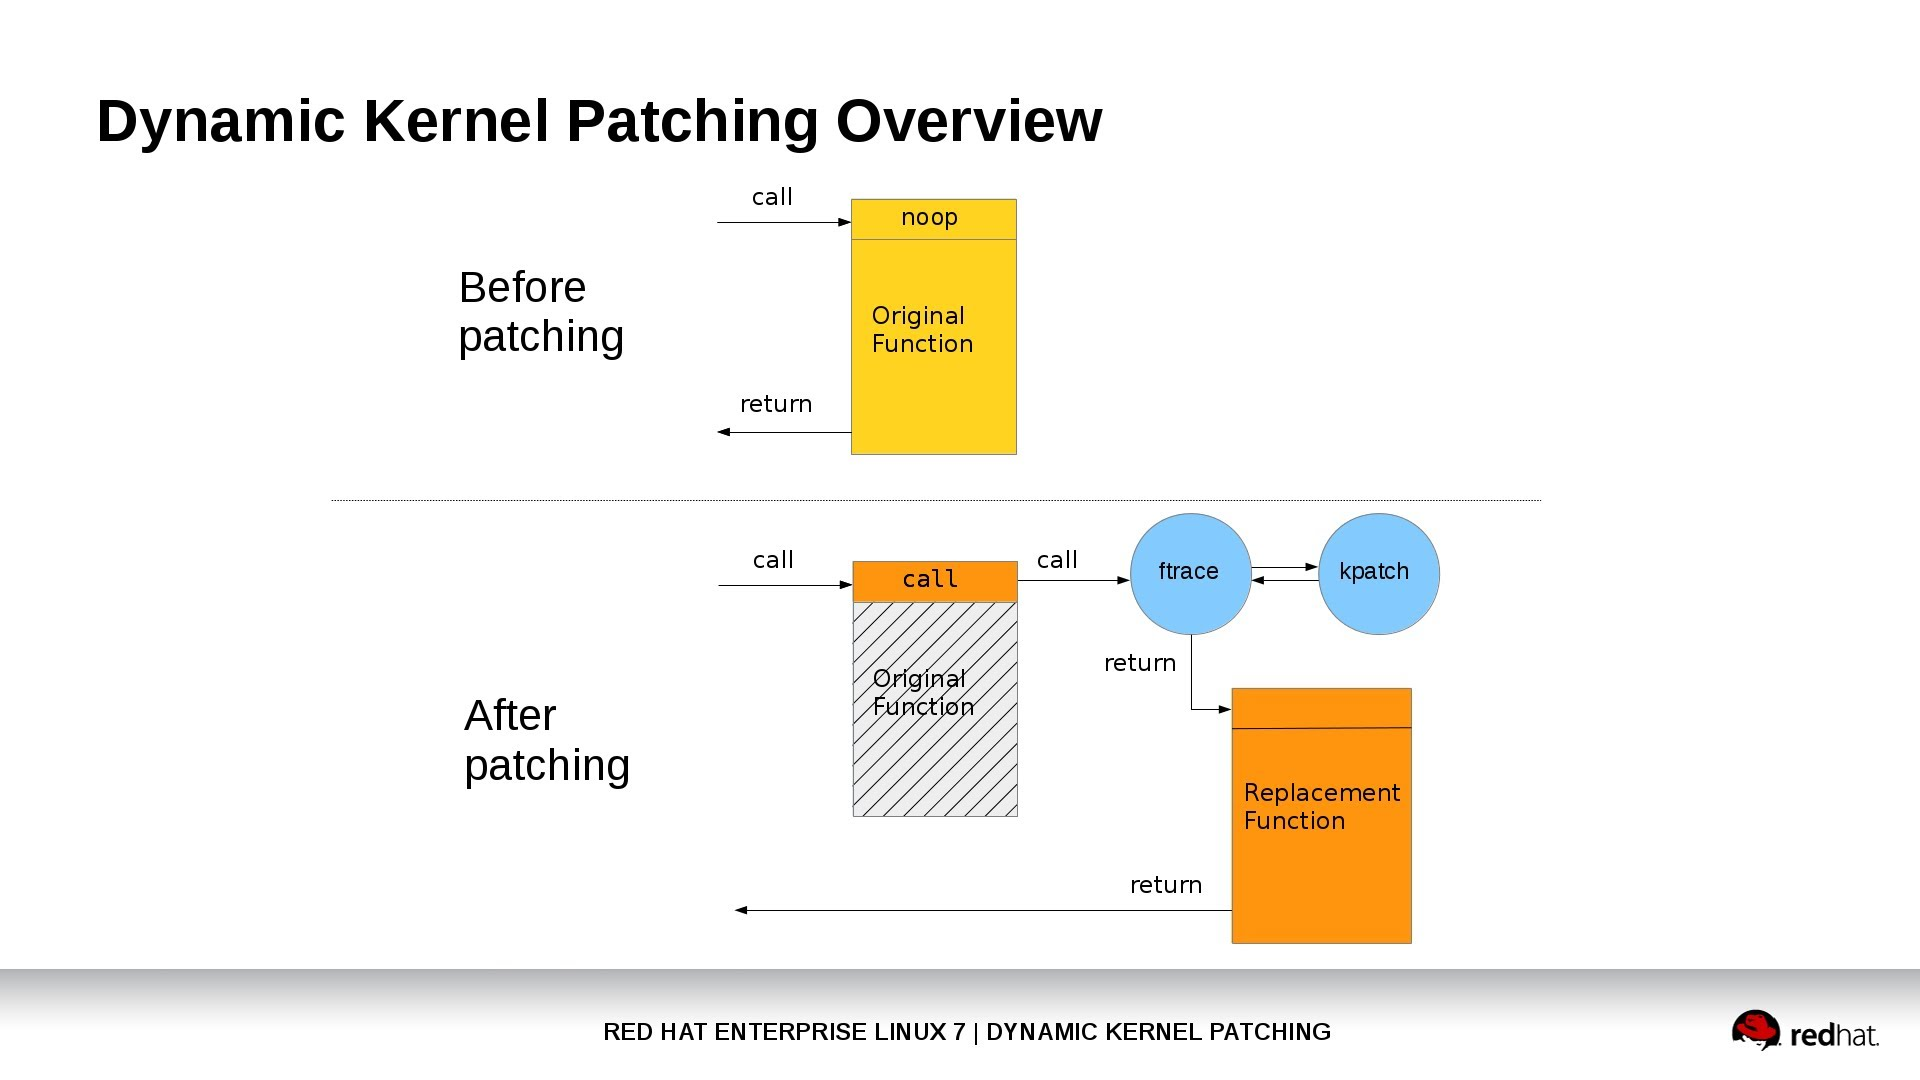
\includegraphics[width = 0.6\textwidth]{kpatch.jpg}
		\caption{Kpatch \cite{kpatch}}
	\end{figure}
\end{frame}
\begin{frame}[allowframebreaks]{Bibliografia}
  \begin{thebibliography}{9}
    \setbeamertemplate{bibliography item}[online]
  \bibitem{ELFPic}{ \url{http://www.cirosantilli.com/elf101.png} }
  \bibitem{kpatch}{ \url{https://github.com/dynup/kpatch} }
    \setbeamertemplate{bibliography item}[article]
  \bibitem{ar1}{ \url{http://www.lurklurk.org/linkers/linkers.html} }
  \bibitem{ar2}{
      \url{https://carsontang.github.io/unix/2013/06/01/guide-to-object-file-linking/}
    }
  \bibitem{ar3}{ \url{http://www.skyfree.org/linux/references/ELF_Format.pdf} }
  \bibitem{ar4}{
      \url{https://www.symantec.com/connect/articles/dynamic-linking-linux-and-windows-part-one}
    }
  \bibitem{ar5}{
      \url{https://en.wikipedia.org/wiki/Executable_and_Linkable_Format} }
  \end{thebibliography}
\end{frame}

\end{document}
